\chapter{Einleitung}


- Lernendes Subjekt = Agent\\
- Zielorientierte Interaktion mit einer Umgebung\\
- Trial and Error Search und Delayed Reward als Erkennungsmerkmale\\
- Trade Off zwischen Exploration und Explotation







\iffalse

% Kapazitätstrends und Limits in optischen Kommunikationsnetzen \cite{Essiambre2012}\\
% Über die Durchbrüche auf dem Gebiet der optischen Netze im Jahr 2012 gibt \cite{Essiambre2013} einen
% Überblick. Viel verspricht man sich durch räumliches Multiplexen; neben Modenmultiplex auch durch den
% Einsatz von Mehrkernfasern.


Optische Kommunikationsnetze bilden bis heute die unangefochtene Grundlage für die Übertragung großer Datenmengen über weite Strecken bei gleichzeitig geringer Latenz.
Damit ist die optische Übertragungstechnik die Grundlage moderner Kommunikationsnetze und insbesondere des Internets.
Erste kommerzielle optischen Übertragungssysteme stellten gerade einmal eine Übertragungskapazität von weniger als \SI{100}{\mega\bit\per\second} zur Verfügung.\par\medskip
Die durchschnittliche Last am deutschen Internetknoten DE-CIX ist in Abbildung \ref{fig:DE-CIX} dargestellt. Derzeit liegt diese bei über \SI{1,4}{\tera\bit\per\second}.

\begin{figure}[ht!]
 \centering
 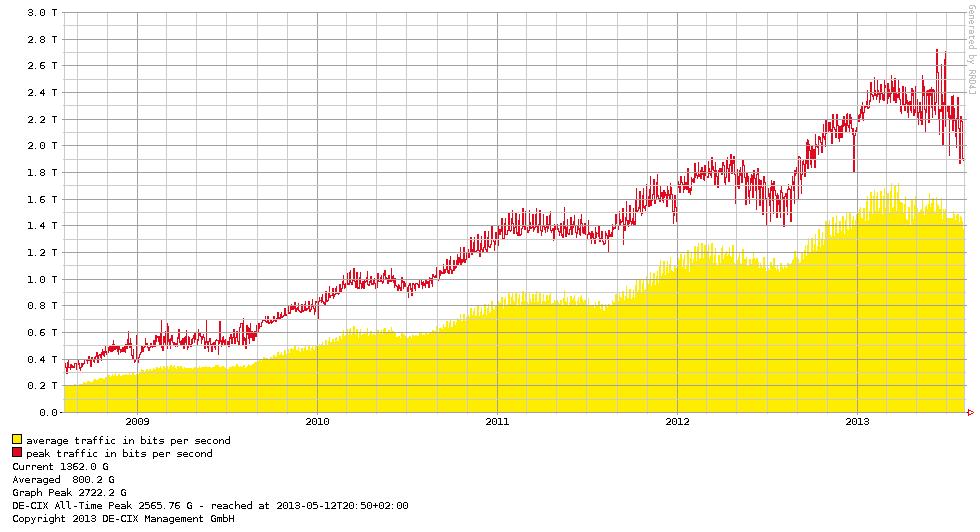
\includegraphics[keepaspectratio,width=0.9\textwidth]{abbildungen/de-cix_5y_20130804.png}
 \caption{DE-CIX Traffic Statistik, 5 Jahres Grafik \protect\footnotemark[1]}
 %\caption{DE-CIX traffic statistics, 5 year graph \protect\footnotemark[1]}
 \label{fig:DE-CIX}
\end{figure}

\footnotetext[1]{\url{http://www.de-cix.net/about/statistics/}}

Eine verständliche Einführung in die Tiefen der optischen Übertragungstechnik bietet das Vorlesungsskript OUET \cite{ouet}.
Eine weitere wichtigste Quellen ist \cite{Agrawal2012}.



\section{Abkürzungen}
Für Abkürzungen kann das Paket \textit{acronym} verwendet werden.
Ein Abkürzungsverzeichnis ist nicht erforderlich, sofern alle Akbürzungen bei der ersten Verwendung eingeführt werden.
Dies wird durch die Verwendung von \textit{acronym} vereinfacht, jedoch ist die Nutzung des Paketes rein optional.
Das Paket bietet folgende Optionen (siehe  \LaTeX~Quelltext):\par\medskip
\begin{itemize}
 \item \ac{NLSE}         % fügt die Abkürzung ein, außer beim ersten Aufruf, hier wird die Erklärung mit angefügt
 \item \acs{NLSE}        % fügt die Abkürzung ein
 \item \acf{NLSE}        % fügt die Abkürzung UND die Erklärung ein
 \item \acl{NLSE}        % fügt nur die Erklärung ein
\end{itemize}



\section{Mathematik}
Für mathematische Formeln wird das \textit{amsmath} Paket verwendet. Gleichungen sind damit recht schön zu setzen:

\begin{equation}
\frac{{\partial A}}{{\partial z}} =  - \frac{\alpha }{2}A + i{\beta ^{(0)}}A - {\beta ^{(1)}}\frac{{\partial A}}{{\partial t}} - i\frac{{{\beta ^{(2)}}}}{2}\frac{{{\partial ^2}A}}{{\partial {t^2}}} + i\gamma {\left| A \right|^2}A
\label{equ:nlse}
\end{equation}

Auch das Referenzieren von Gleichungen ist recht einfach. Dabei ist mit Gleichung \eqref{equ:nlse} eine mögliche Darstellungsform der \acs{NLSE} gegeben.

\fi
